\documentclass[11pt]{article}
\usepackage[utf8]{inputenc}
\usepackage[a4paper, landscape, margin=1cm]{geometry}
\usepackage{multicol}
\usepackage{lato}
\usepackage{graphicx}
\usepackage{enumitem}
\usepackage[dvipsnames, svgnames]{xcolor}
\usepackage{tcolorbox}
\usepackage{needspace}
\tcbuselibrary{skins, breakable}

% --- Settings ---
\pagestyle{empty}
\definecolor{SmaileBlue}{HTML}{00AEEF}
\definecolor{SmaileGreen}{HTML}{92D050}
\definecolor{SmaileOrange}{HTML}{ED7D31}
\definecolor{SmaileGray}{HTML}{595959}
\definecolor{SmaileLightBlue}{HTML}{E7F7FE}
\definecolor{SmaileLightGreen}{HTML}{F4FBEE}

\newcommand{\pamphletheading}[1]{%
  \par
  \needspace{4\baselineskip} 
  \noindent{\Large\bfseries\color{SmaileGreen}#1}%
  \par\vspace{1ex}%
  \nopagebreak 
}

\begin{document}
\color{SmaileGray}

\begin{multicols}{3}
% --- Panel 1: Intro (Inner Flap) ---
\pamphletheading{Introduction}
Where does our food come from? 

In this workshop, children (4-7) will visit "Farmer Ella's Smart Farm" to learn how robots and smart computers (AI) help grow delicious apples, carrots, and lettuce.

\vfill\null
\pamphletheading{Key Goals}
\begin{tcolorbox}[colback=SmaileLightGreen, colframe=SmaileGreen, boxrule=0.5pt, arc=2mm]
\small
\begin{itemize}[leftmargin=*]
    \item \textbf{Explore:} How food is grown on smart farms.
    \item \textbf{Understand:} AI as a helper.
    \item \textbf{Role-Play:} Act as robots and AI brains.
    \item \textbf{Create:} Design a future food robot.
\end{itemize}
\end{tcolorbox}

% --- Panel 2: Back (Resources) ---
\columnbreak
\pamphletheading{Resources}
\begin{itemize}
    \item \textbf{Story:} "Farmer Ella and the Robot Helpers".
    \item \textbf{Props:} Watering cans, fruit baskets.
    \item \textbf{Art:} Crayons, paper, coloring sheets.
    \item \textbf{Support:} Teacher-led slides or picture prompts.
\end{itemize}

\vfill\null
\centering

\includegraphics[height=1.5cm]{smaile_brand_assets/Logo_Co-founded_by_EU.jpeg}
\par\tiny 
Co-funded by the European Union.

% --- Panel 3: Front Cover ---
\columnbreak
\centering
\vspace*{2cm}

\includegraphics[height=3cm]{smaile_brand_assets/logo_smaile_transparentbg_no_smaile.png}
\vspace{1cm}
\par
{\Huge\bfseries\color{SmaileGreen} A Bite of Future}
\vspace{0.5cm}
\par
{\Large Smart Farms \& Robots}
\vspace{2cm}
\par
Target Group: 4-7 y.o.
\par
\textbf{SmAIle Project}

\end{multicols}
\newpage

\begin{multicols}{3}
% --- Panel 4: Outcomes (Inside Left) ---
\pamphletheading{Learning Outcomes}
\begin{tcolorbox}[colback=SmaileLightBlue, colframe=SmaileBlue, boxrule=0.5pt, arc=2mm]
\small
\textbf{Knowledge:}
\begin{itemize}[leftmargin=*]
    \item Recognize tasks machines can do (watering, picking).
    \item Understand AI helps make decisions.
\end{itemize}
\textbf{Skills:}
\begin{itemize}[leftmargin=*]
    \item Role-playing \& Drama.
    \item Simple cause-and-effect logic.
    \item Creative Drawing.
\end{itemize}
\end{tcolorbox}

\vspace{1em}
\pamphletheading{Values}
\begin{tcolorbox}[colback=SmaileLightGreen, colframe=SmaileGreen, boxrule=0.5pt, arc=2mm]
\small
\begin{itemize}[leftmargin=*]
    \item Curiosity about food.
    \item Teamwork.
    \item Valuing technology.
\end{itemize}
\end{tcolorbox}


% --- Panel 5: Activities (Inside Center) ---
\pamphletheading{1. Storytime \& Role-Play}
We read \textit{Farmer Ella and the Helpful Robots} and meet Picksy, Sprinkles, and Brainy.

\begin{center}
    % Insert Farmer Ella Image here
    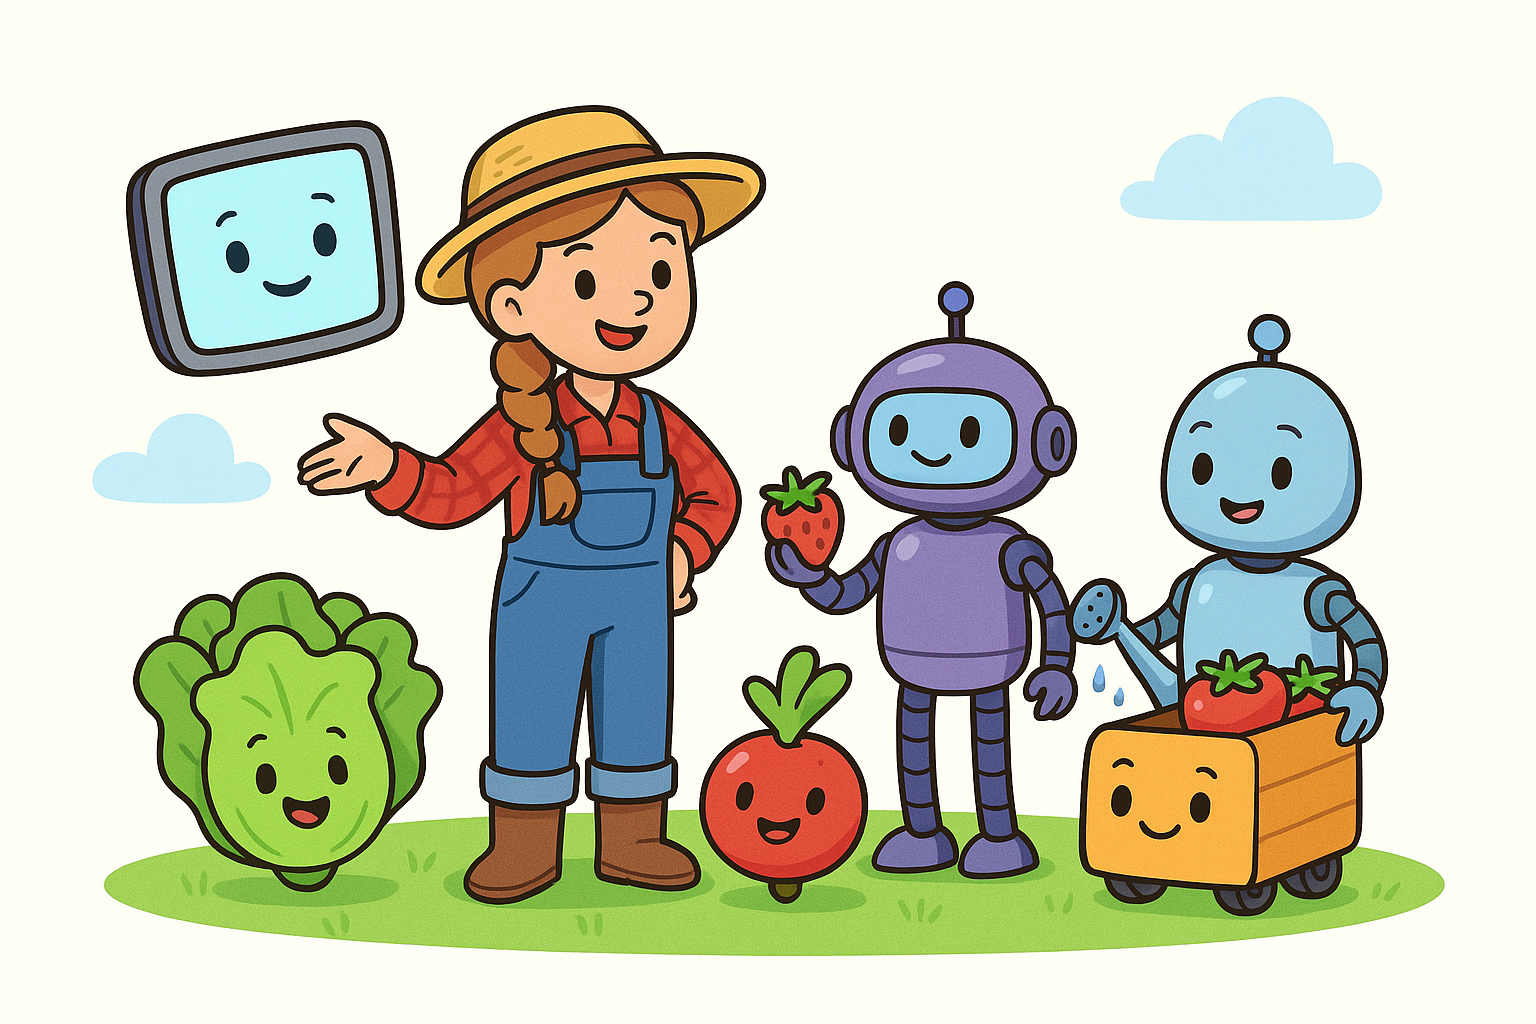
\includegraphics[width=0.9\linewidth]{images/scenario_bite_future_4-7_img1.png}
\end{center}

\textbf{Smart Farm Simulation:}
Children take on roles of Plants, Robots, and AI. The "AI" gives instructions based on weather cues: \textit{"It's raining! Don't water the plants!"}

% --- Panel 6: Creative (Inside Right) ---
\pamphletheading{2. Creative Design}
\textbf{My Food Robot:}
Children use imagination to draw their own robot helper. \textit{"My robot helps by... sorting the carrots!"}

\pamphletheading{3. Reflection}
\begin{tcolorbox}[colback=white, colframe=SmaileOrange, boxrule=0.5pt]
\small
\textbf{Activity:} Color "Brainy the AI"!
\end{tcolorbox}

\begin{center}
    % Insert Brainy AI Coloring Image here
    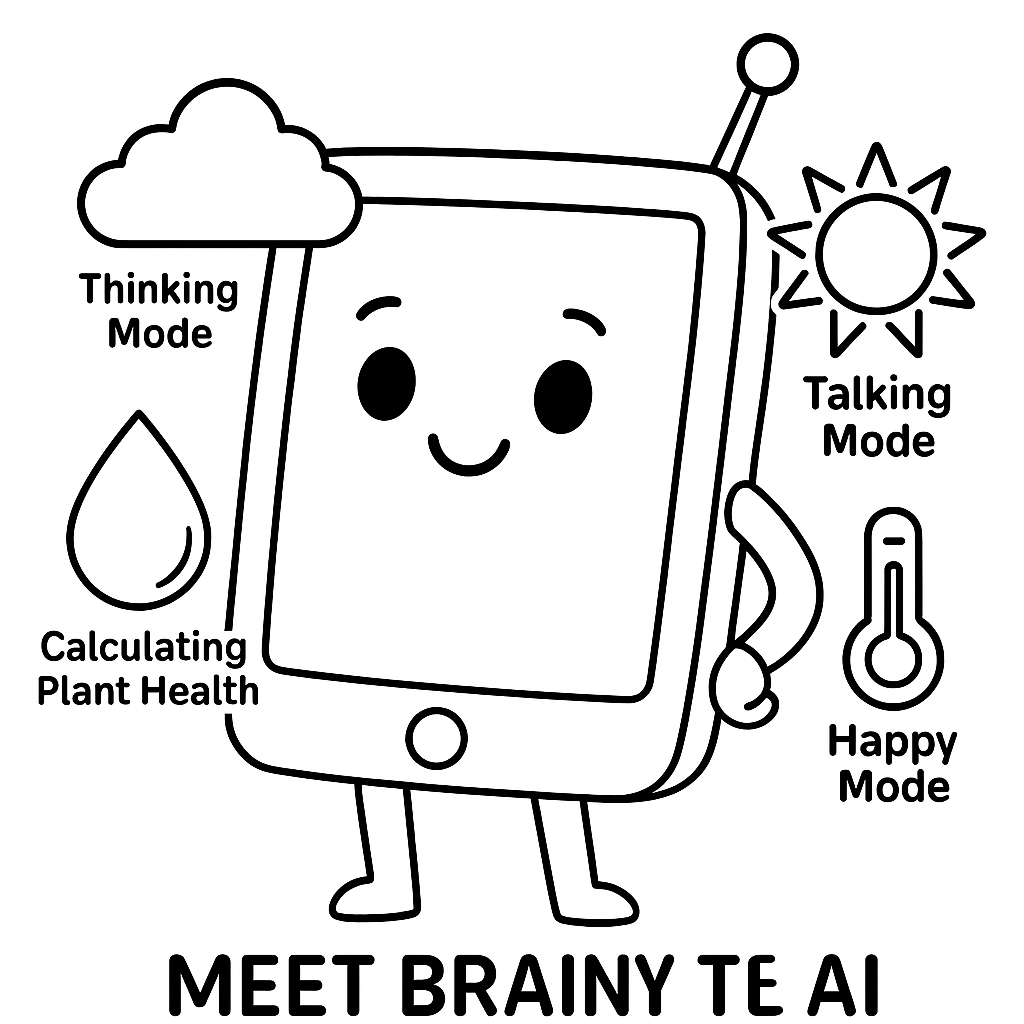
\includegraphics[width=0.7\linewidth]{images/scenario_bite_future_4-7_img2.png}
\end{center}

\end{multicols}
\end{document}
